\subsection{AES algorithm workflow}

\Gls{AES} is a symmetric block cipher that operates on 128-bit blocks of data.
It processes these blocks in several rounds, with each round consisting of multiple layers that manipulate the data in specific ways. 
These layers introduce both \textit{confusion} and \textit{diffusion} to strengthen the encryption.

\subsubsection{Encryption process}

The AES structure consists of the following layers \cite{Paar2024}:
\begin{enumerate}
    \item \textbf{Key Addition Layer}:
    A 128-bit round key is \texttt{XOR} with the state, with round key generated in Key Expansion (Section~\ref{sec:key-expansion}).

    \item \textbf{Byte Substitution Layer (S-Box)}:
    Each byte of the state is non-linearly transformed using lookup tables. 
    This introduces confusion, ensuring that small changes in the input lead to significant, non-linear changes in the output.
    
    \item \textbf{Diffusion Layer}:
    This layer spreads the influence of each byte over the entire block. 
    It is divided into two sub-layers:
    \begin{enumerate}
        \item \textbf{\textsc{ShiftRow} Layer}: The rows of the state are shifted cyclically, which helps spread the data. %permutes the data on a byte level
        \item \textbf{\textsc{MixColumn} Layer}: This layer performs a matrix multiplication operation on the columns of the state, mixing the data across the block. % is a matrix operation which combines/mixes blocks of four bytes. 
    \end{enumerate}
\end{enumerate}

Each round, except the initial round, consists of all three layers. 
The initial round consists of only the Key Addition layer.
The final round omits the \textsc{MixColumn} transformation, making both encryption and decryption operations symmetric.
Figure \ref{fig:aes-block-diagram} shows the block diagram of AES encryption.

\begin{figure}[!ht]
    \centering
    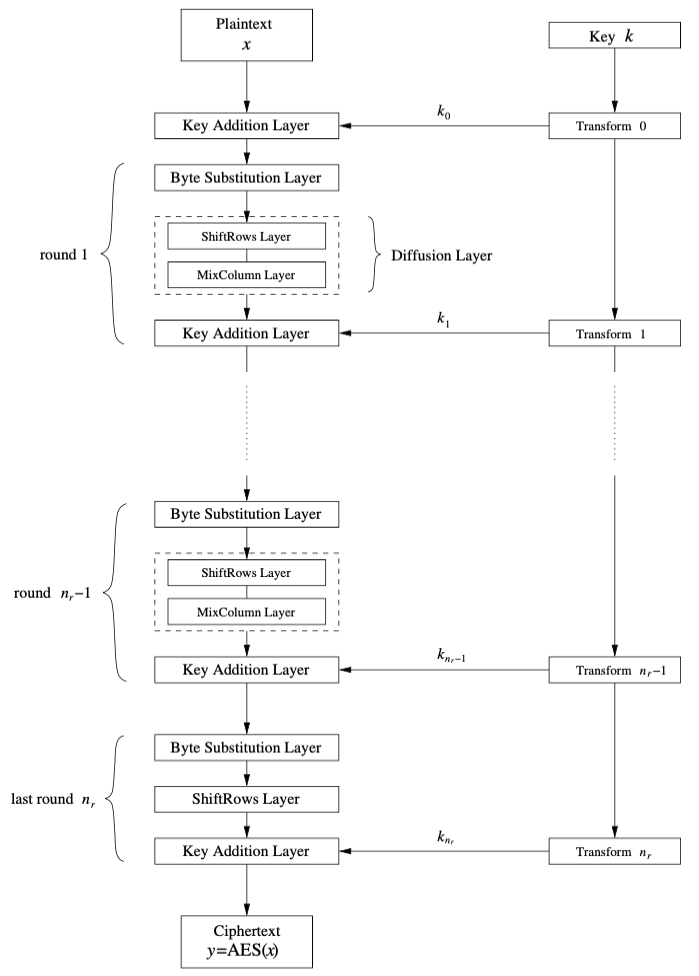
\includegraphics[width=.8\textwidth]{aes-block-diagram.png} % Adjust width as needed
    \caption{
        AES Encryption Block Diagram \cite{Paar2024}.
        The plaintext is denoted as $x$, the ciphertext as $y$, key as $k$, and the number of rounds as $n_r$.
    }
    \label{fig:aes-block-diagram}
\end{figure}


\subsubsection{Decryption process}
\label{sec:decryption}

AES decryption is the process of reversing encryption steps to retrieve the original plaintext from a given ciphertext. 
Since AES is a symmetric block cipher, it uses the same secret key for both encryption and decryption \cite{NIST_AES}.

The input data is handled in 128-bit blocks and processed through multiple transformation rounds. 
The number of rounds depends on the key size, as outlined in Table \ref{table:key-length-rounds}.

To decrypt, AES performs the inverse of each encryption step, but in reverse order. These inverse operations are:

\begin{enumerate}
    \item \textbf{AddRoundKey}: This step \texttt{XOR} the block with the corresponding round key. Since \texttt{XOR} is its own inverse, this operation is identical in both encryption and decryption.
    \item \textbf{InvMixColumns}: Reverses the mixing of bytes in each column. This step is skipped in the final round.
    \item \textbf{InvShiftRows}: Reverses the row shifts that were applied during encryption.
    \item \textbf{InvSubBytes}: Applies the inverse S-box substitution to each byte, undoing the non-linear transformation.
\end{enumerate}

Decryption starts by XORing the ciphertext with the final round key. 
Then, each round applies the inverse transformations using the appropriate round key from the key schedule. 
After all rounds are completed, the original plaintext is recovered.
